\section{Diseño y resolución}

En esta sección se documentará el trabajo realizado de cara al desarrollo y resolución del proyecto durante las distintas fases por las que este ha ido pasando.

\subsection{Prueba de modelo generalista}

Antes de acometer el desarrollo de un proyecto de \textit{deep learning}, conviene mirar a las soluciones que ya existen y si estas pueden ser útiles para nuestro problema. OpenCV, como hemos visto, aporta multitud de algoritmos que pueden utilizarse para hacer un seguimiento visual o \textit{tracking} de un objeto, en nuestro caso, del balón.

Entre estos algoritmos se encuentra GOTURN, cuyas siglas significan \textit{Generic Object Tracking Using Regression Networks}, que fue propuesto en un artículo de \citet{art:goturn}. La mayor aportación de este algoritmo respecto de otros enfoques más clásicos (por ejemplo, Meanshift y Camshift), es que el aprendizaje sobre el objeto a seguir se ocurre antes del tiempo de ejecución, de forma que durante la ejecución no se realiza aprendizaje de ningún tipo, como se ve en la figura \ref{fig:goturn1}.

\begin{figure}[H]
  \centering
  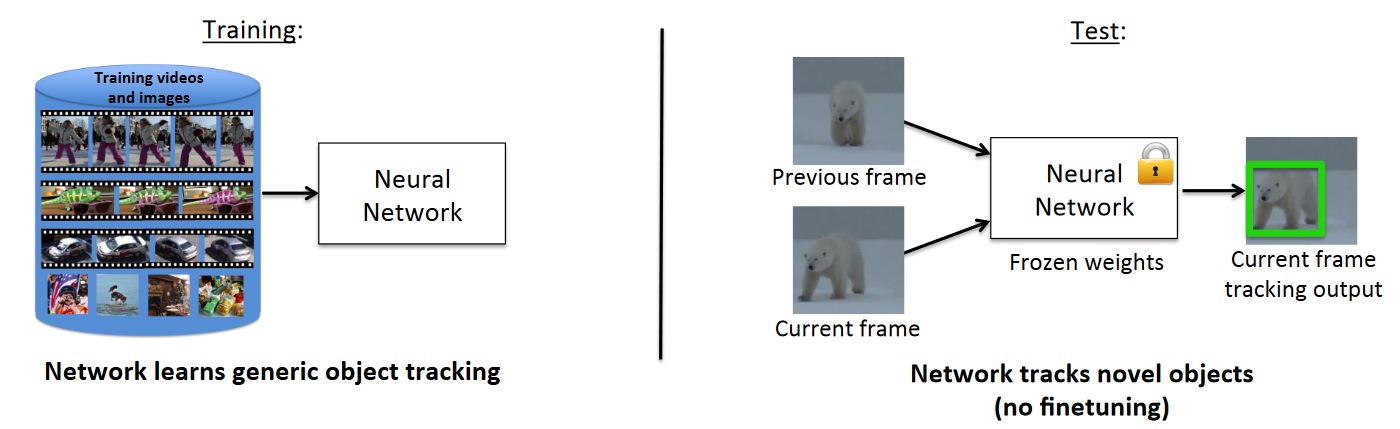
\includegraphics[width=0.6\textwidth]{images/goturn}
  \caption{Esquema del modelo GOTURN diferenciando entre entrenamiento y test \cite{art:goturn}.}
  \label{fig:goturn1}
\end{figure}

Este enfoque permite que GOTURN sea más rápida en tiempo de ejecución (en el artículo original se hablaba de 100 FPS), a cambio de que todos aquellos objetos que no se encuentren en el dataset funcionen algo peor (una diferencia de un 10\% de error aproximadamente, según el propio artículo). El dataset sobre el que se entrenó GOTURN es ALOV300++, en el que se incluyen tanto personas como balones, entre otros muchos objetos.

Dado que podemos contar con que el objeto que queremos seguir (el balón) se encuentra en el dataset de entrenamiento, puede ser interesante ver cómo se comporta el modelo en un caso de vídeo real. La implementación de OpenCV requiere descargar el modelo y seleccionar una región de interés para comenzar el seguimiento.

En la figura \ref{fig:goturn2} podemos ver una secuencia de imágenes (tomadas cada 15 frames, o 0.5s) donde se ve el desempeño del modelo en una situación de seguimiento del balón. Como puede verse, el seguimiento se pierde a los pocos segundos y nunca vuelve a recuperarse, el modelo acaba abarcando el campo completo. Este error puede deberse al tamaño reducido del balón en la imagen, unido a lo rápido de su movimiento en ocasiones. Otro error que llama la atención es que el modelo no es capaz tampoco de seguir a ninguna jugadora, probablemente porque las imágenes con las que fue entrenado no incluían personas vistas desde arriba.

\begin{figure}
  \begin{tabular}{cccc}
    \subfloat{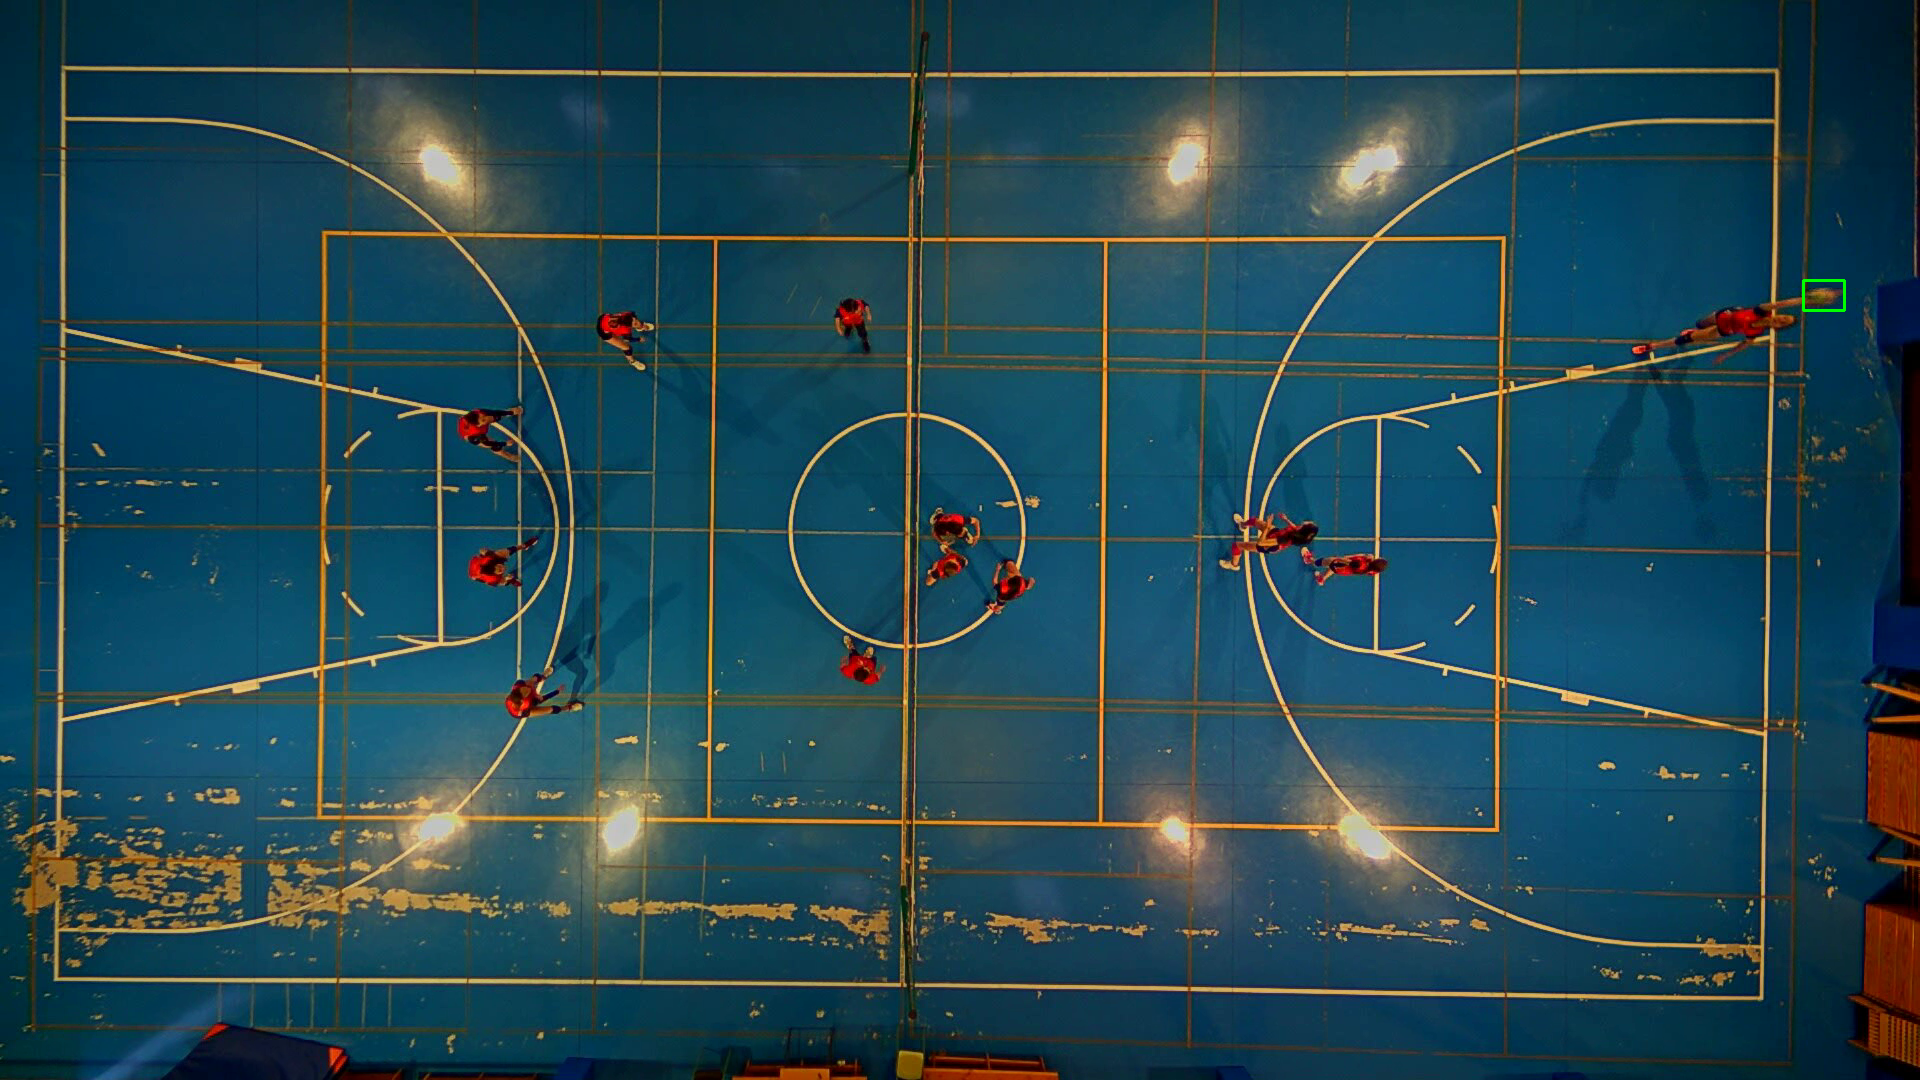
\includegraphics[width = 7.5cm]{images/got1}} &
    \subfloat{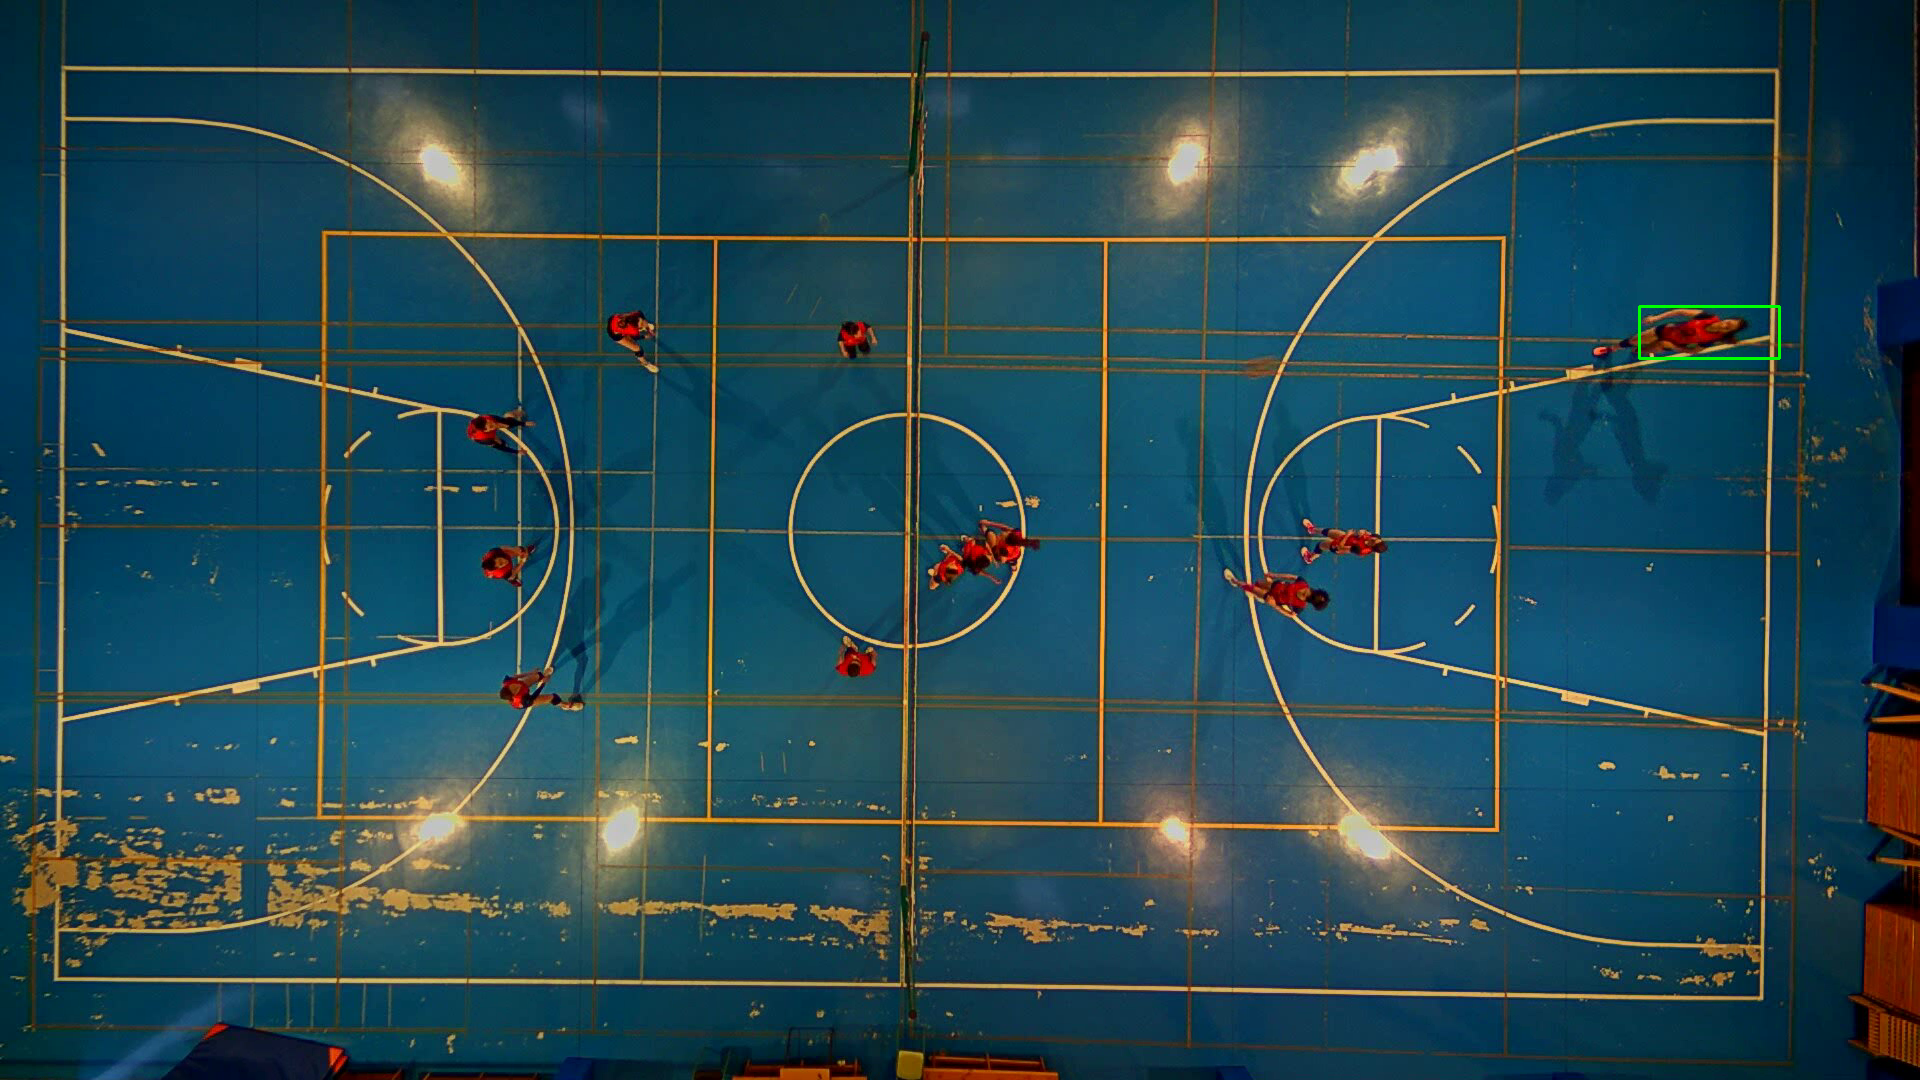
\includegraphics[width = 7.5cm]{images/got2}}   \\
    \subfloat{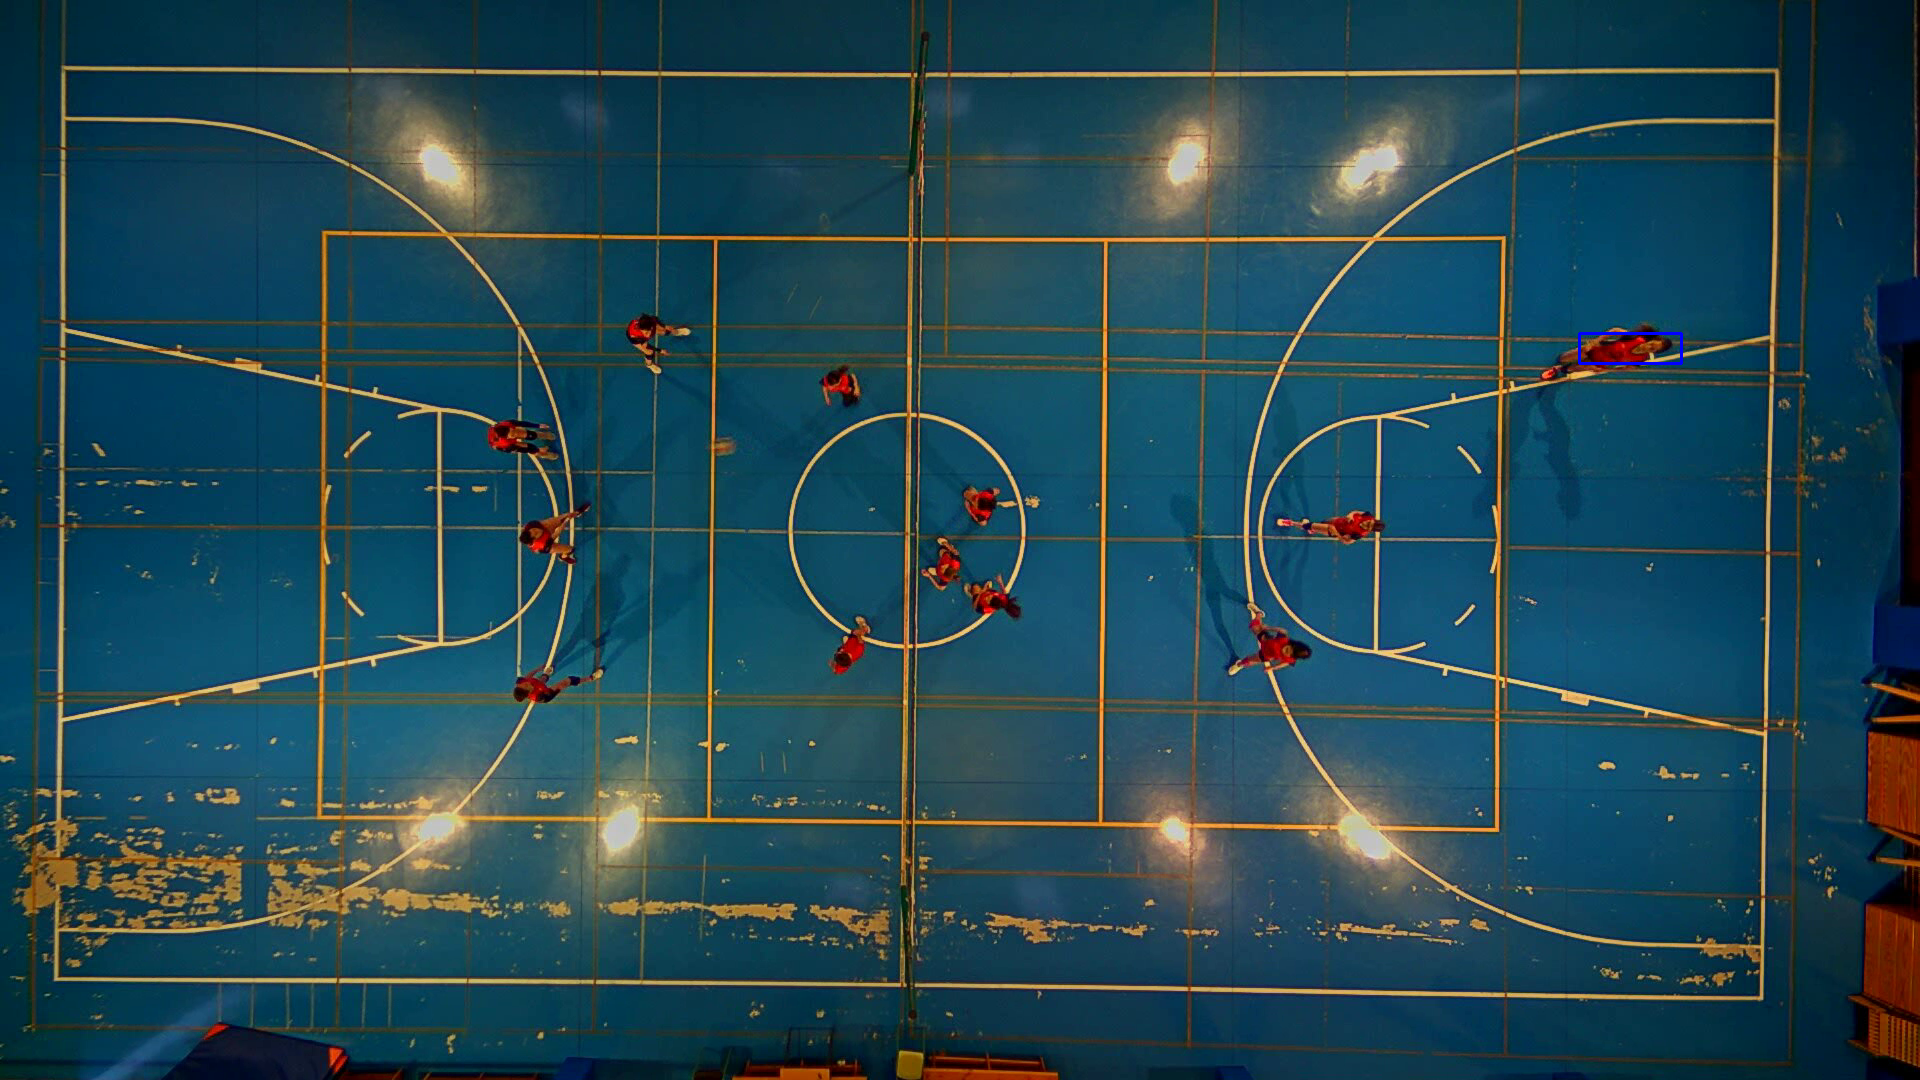
\includegraphics[width = 7.5cm]{images/got3}} &
    \subfloat{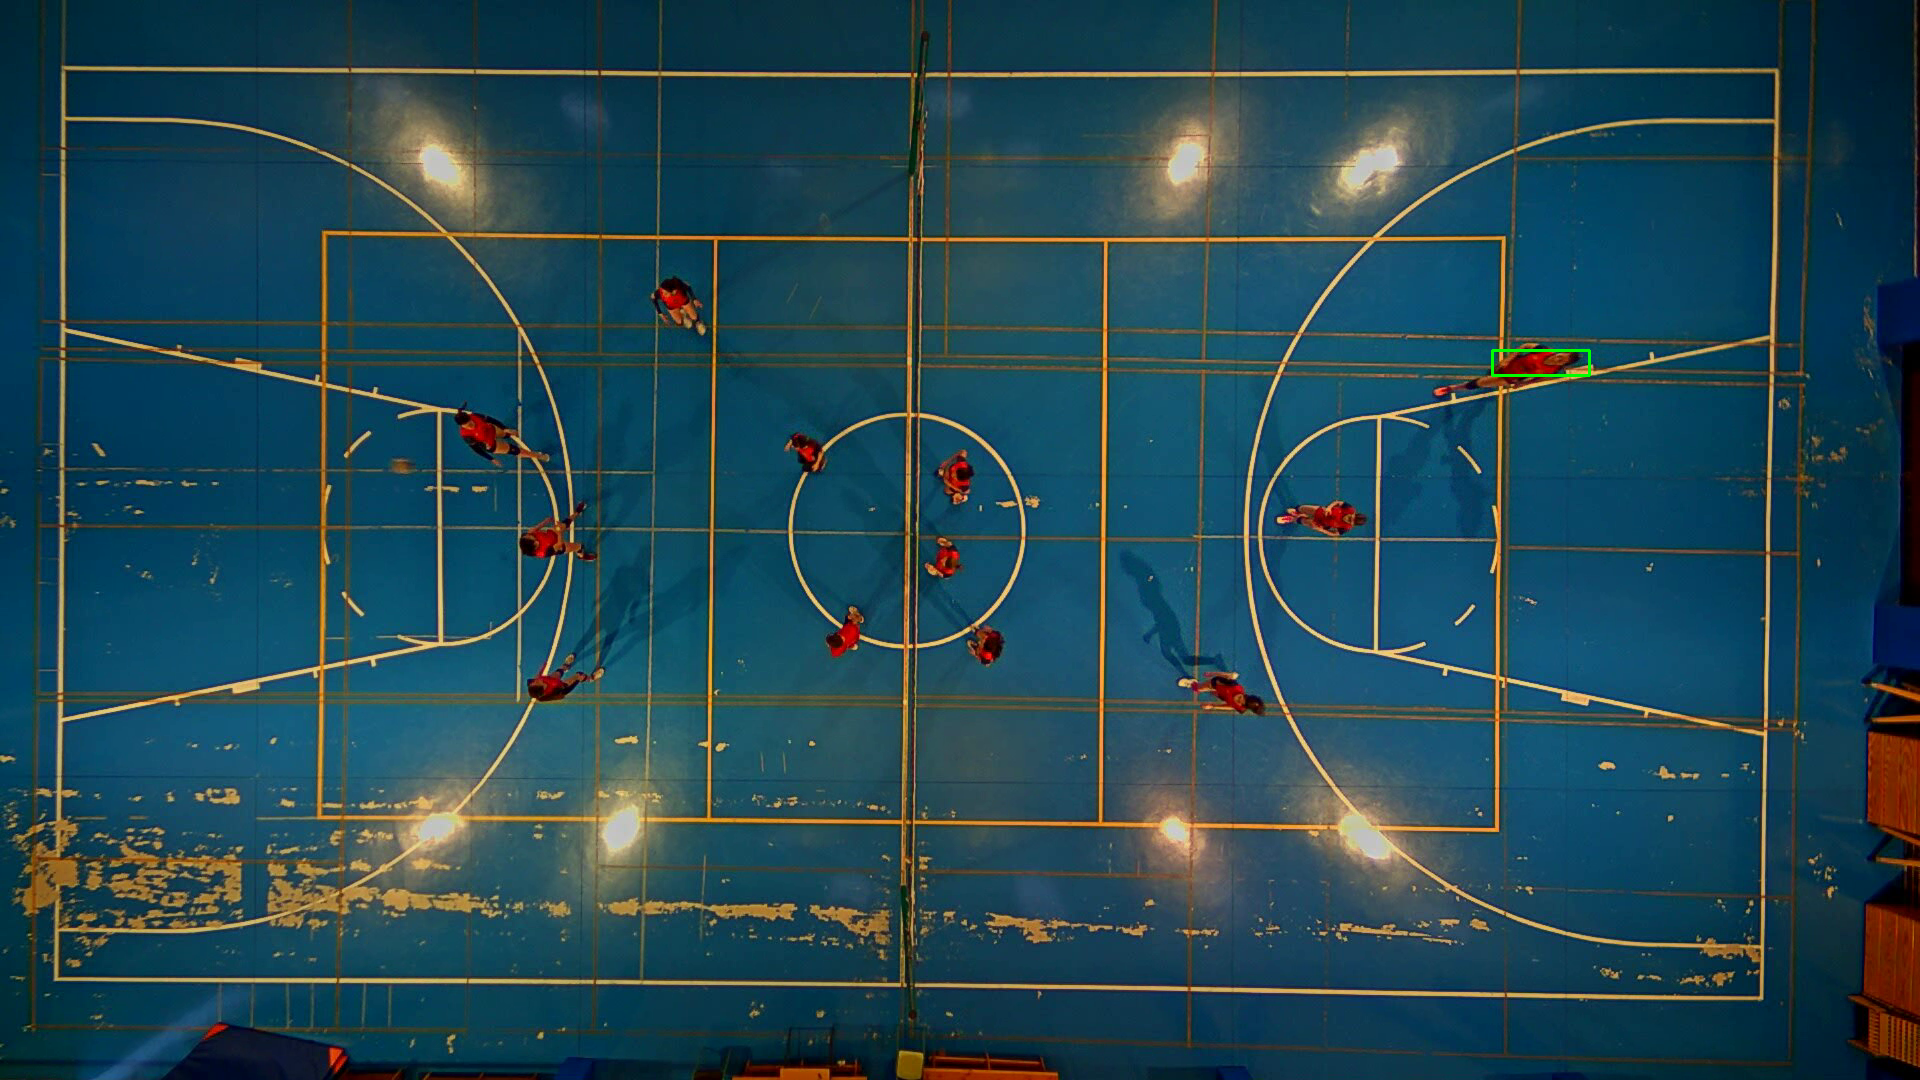
\includegraphics[width = 7.5cm]{images/got4}}   \\
    \subfloat{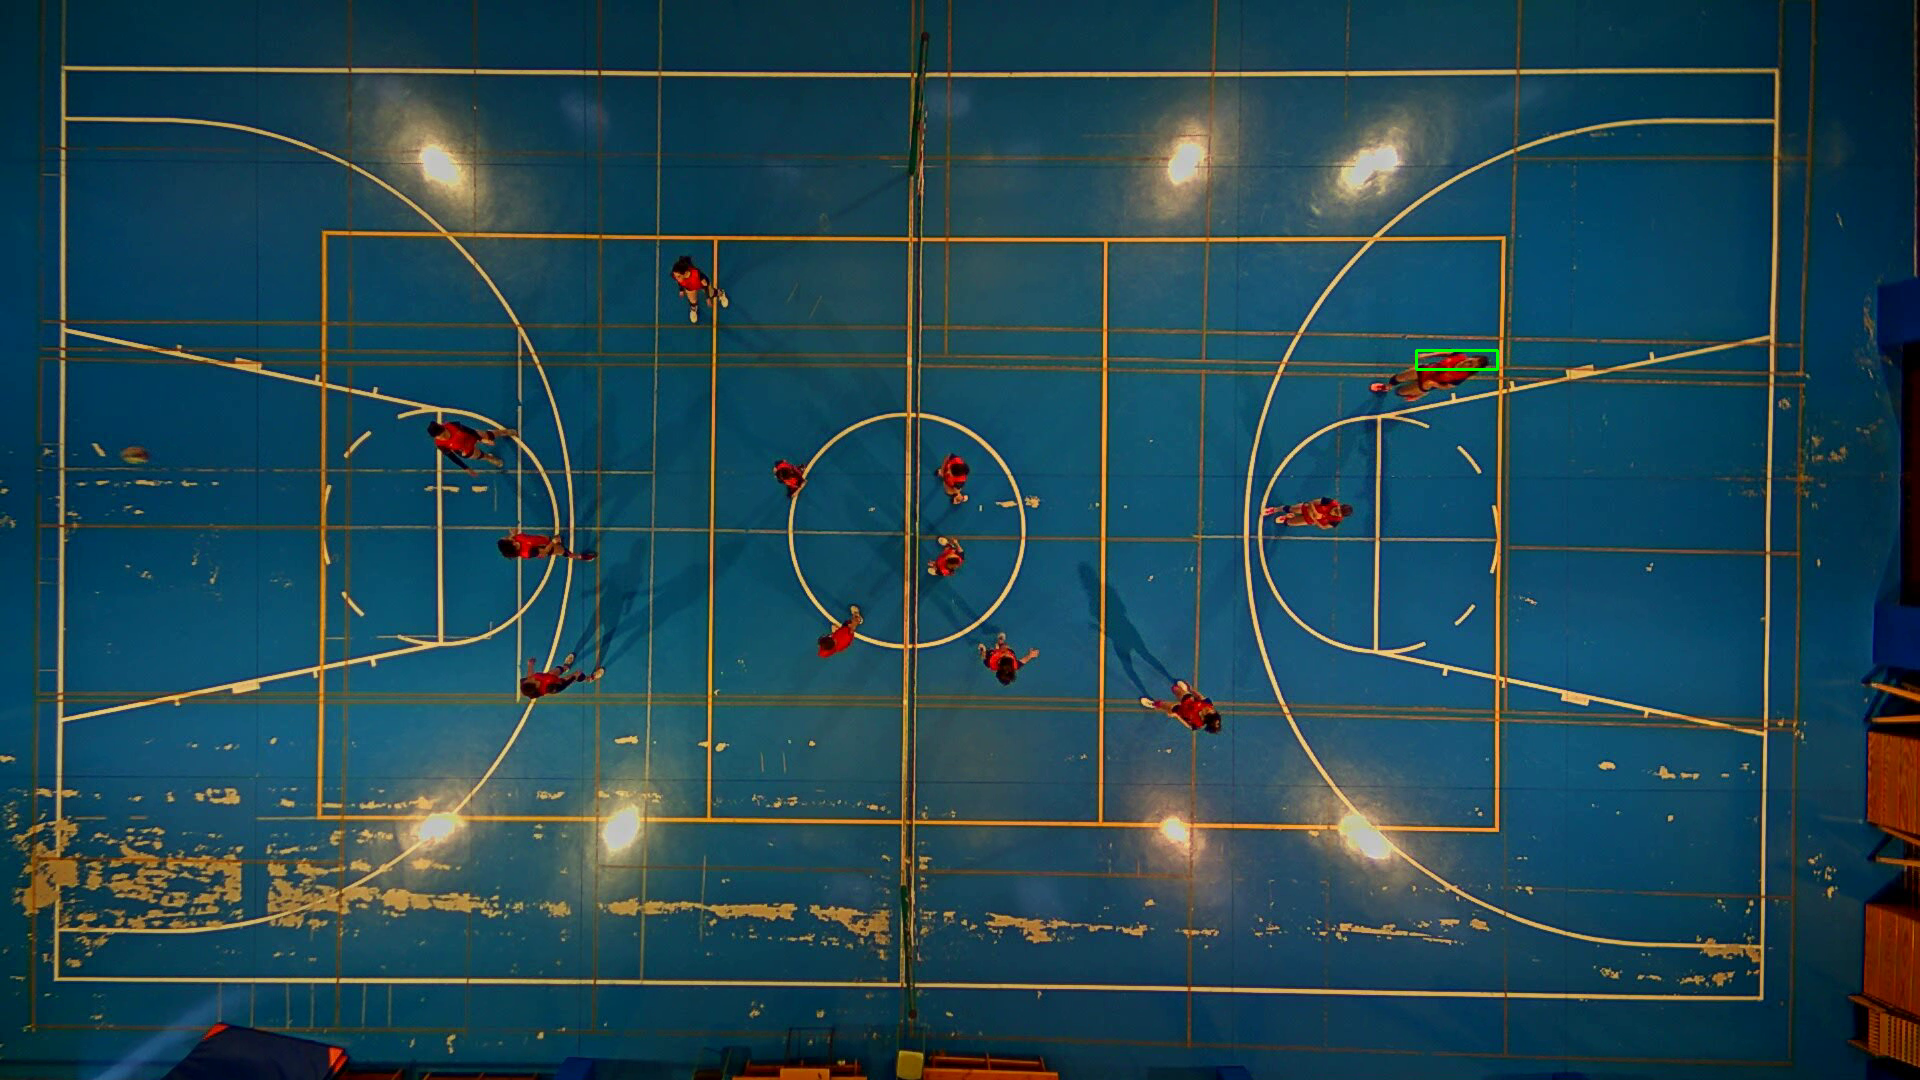
\includegraphics[width = 7.5cm]{images/got5}} &
    \subfloat{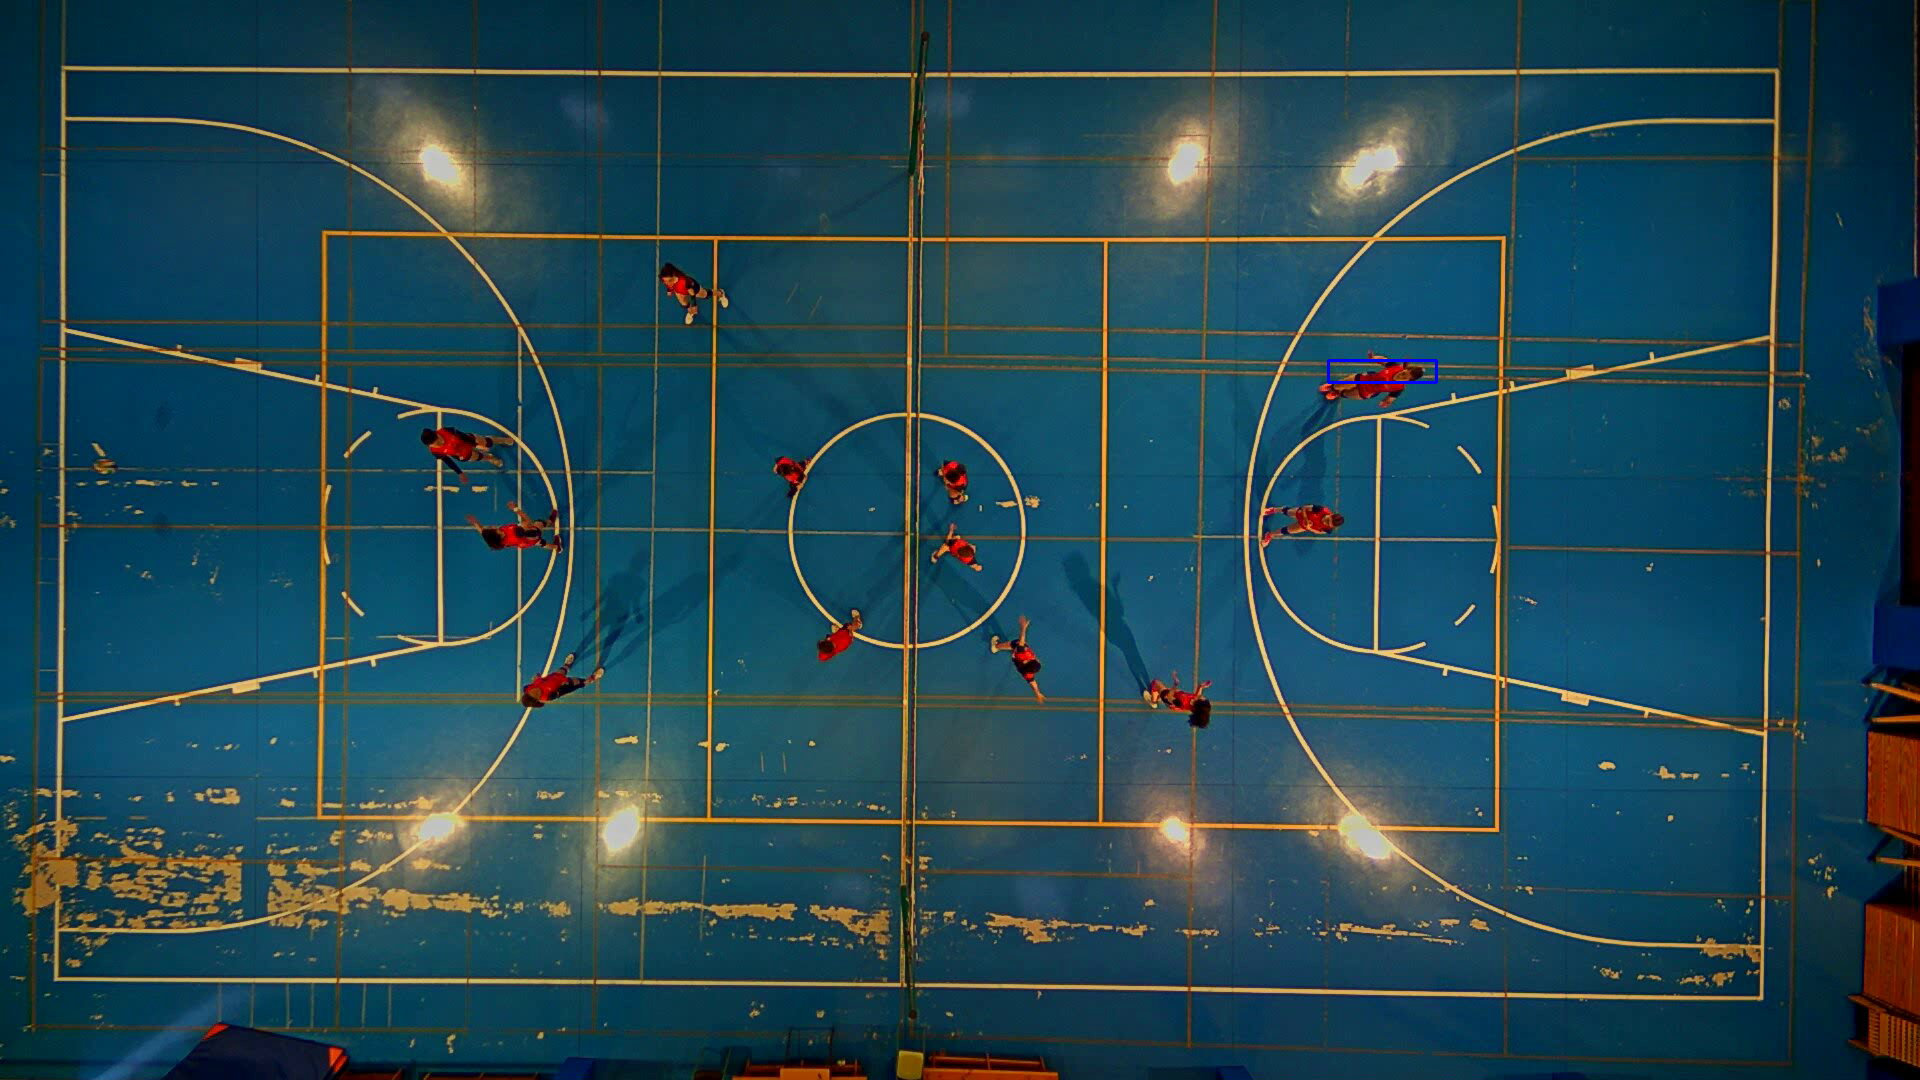
\includegraphics[width = 7.5cm]{images/got6}}   \\
    \subfloat{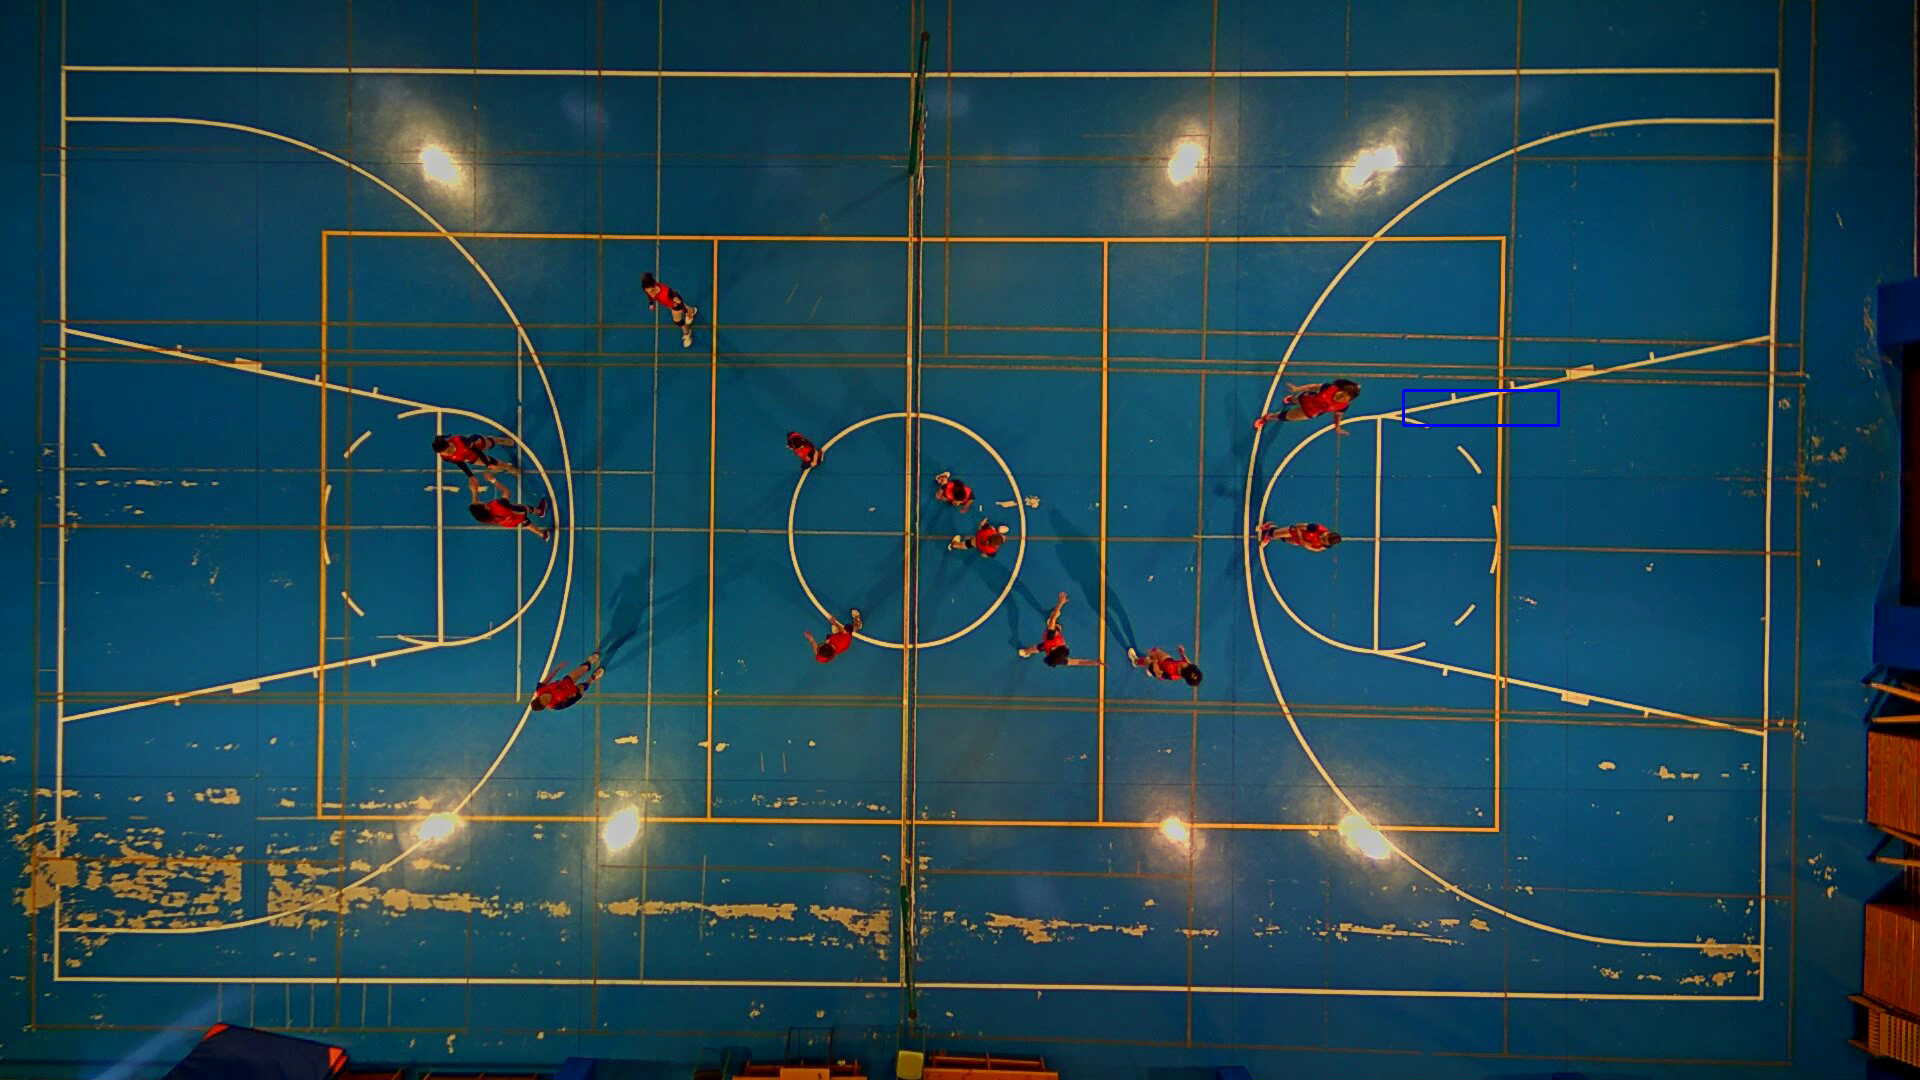
\includegraphics[width = 7.5cm]{images/got7}} &
    \subfloat{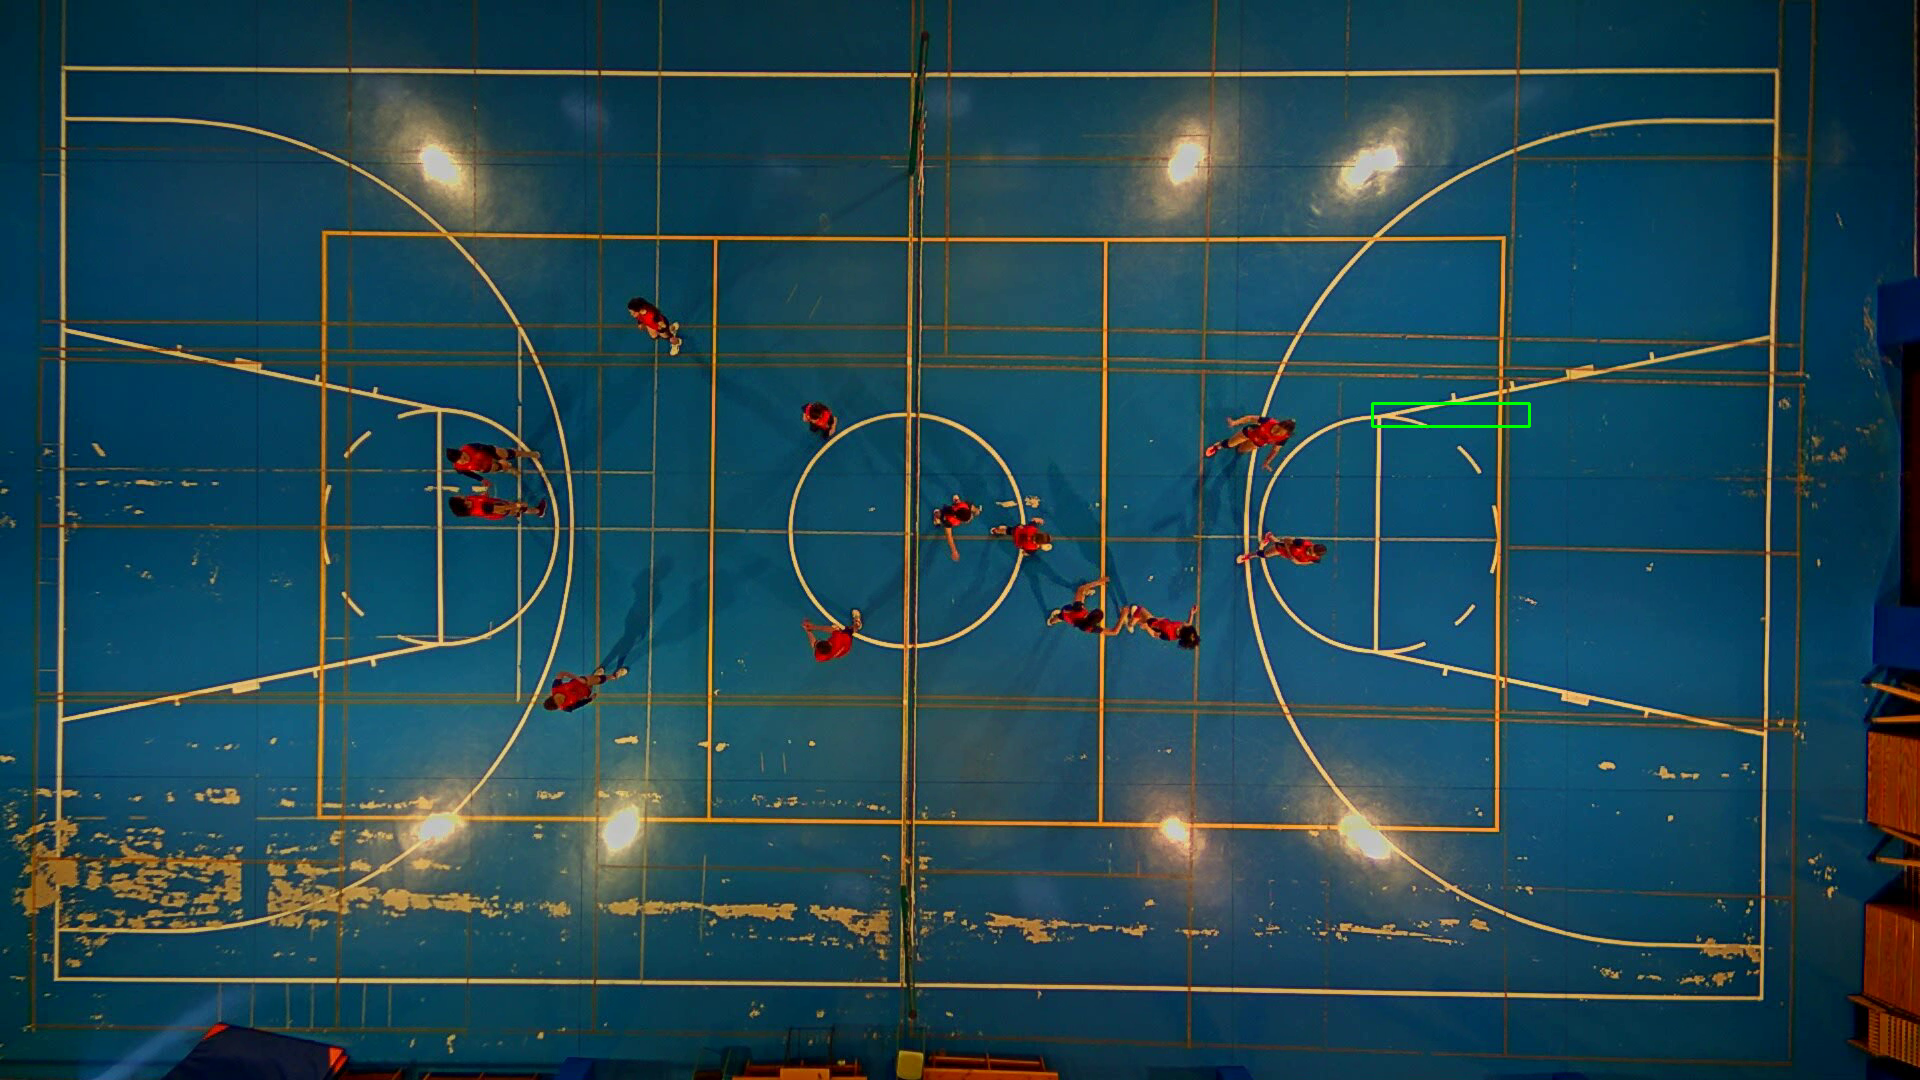
\includegraphics[width = 7.5cm]{images/got8}}
  \end{tabular}
  \caption{Secuencia ejemplo de seguimiento por GOTURN}
  \label{fig:goturn2}
\end{figure}

En conclusión, el tracker genérico de GOTURN no tiene un rendimiento excesivamente bueno, en parte porque nuestro problema es lo suficientemente específico como para necesitar una solución propia. Por ello, tendrá que crearse un modelo propio que desempeñe la tarea que necesitamos: el seguimiento del balón. Para ello, primero habrá que extraer un conjunto de imágenes suficientemente grande a partir de los vídeos con que contamos.

\subsection{Extracción de un dataset a partir de vídeos reales}

Lo primero que deberíamos definir antes de empezar a recoger ejemplos de entrenamiento es la forma preferente que debería tener el dataset resultante. Dado que el objetivo del modelo es predecir la presencia o ausencia de balón en un parche, los ejemplos deberían ser de 2 clases: con balón (positivas) y sin balón (negativas).

El tamaño del parche de entrenamiento debería ser lo suficientemente grande como para que quepa el balón, incluso cuando esté a cierta altura y tenga un tamaño mayor que el habitual. Este tamaño, dado que el balón acostumbra a ocupar unos 20 píxels en la imagen, puede ser 56x56 píxels.

Para extraer las imágenes se ha seguido una estrategia semiautomática. Utilizando los resultados de mi TFG, el cual tenía como objetivo hacer un seguimiento mediante sustracción de fondo, pueden obtenerse un buen número de ejemplos positivos así como negativos.

\subsubsection*{Parte automática}

Para esta parte, como decíamos, se ha utilizado la salida de mi TFG. Cada 10 frames, se extrae una imagen positiva (si se puede) y una negativa. Para obtener la imagen negativa, no es necesaria una estructura demasiado sofisticada, bastaría con obtener una posición aleatoria de la imagen en la que el detector no haya identificado la presencia de balón y guardarla. Con la suficiente duración de los vídeos (contamos con alrededor de 20 minutos), se pueden obtener de esta forma muestras de casi toda la casuística de negativos posible: manchas del campo, líneas, el propio campo, jugadoras, la red y mobiliario del pabellón.

En cuanto a los positivos, cada 10 frames se obtiene la parte de la imagen que el detector haya identificado como balón. En caso de no existir, se capta en el siguiente frame posible.

Aunque en ambos casos estamos a merced del detector utilizado, este es un problema mucho más acusado cuando buscamos positivos, ya que este no era capaz de detectar el balón en casos de solapamiento entre jugadora y balón. Además, existe una cierta cantidad de falsos positivos derivada de la forma en que se identificaba el balón en aquella solución: se comprobaba la \textit{circularidad} de este sin más, por lo que en algunas situaciones las jugadoras eran identificadas como balón.

\subsubsection*{Parte manual}

Tras procesar los 20 minutos de vídeo de la forma anteriormente descrita, obtenemos un total de 9014 imágenes, de las cuales 6886 son negativas y 2128 son positivas. Sin embargo, como se ha descrito, los positivos contienen una gran porción de errores que no queda otro remedio que comprobar manualmente y depurarlos.

Tras una revisión manual, el dataset queda reducido a 8023 imágenes con 6877 negativas y 1146 positivas. Como decíamos, el problema de los errores ocurre en ambos casos, pero es mucho más notable. Además, hay una cierta parte de la casuística de positivos con la que no se cuenta en este estado del dataset, que son los solapamientos entre jugadoras y balón. Para solucionar este problema, la única solución posible es obtener ejemplos de forma manual de este tipo de casos así como de otros que se hayan podido escapar.

Tras este proceso llegamos a 9526 imágenes de las cuales 6961 son negativas y 2565 son positivas, las cuales serán divididas en una proporción de 80\% al conjunto de entrenamiento y 10\% a los conjuntos de validación y test. Esta cifra, aunque es razonablemente alta, no nos garantiza que el modelo que se desarrolle sea capaz de extraer las características relevantes de cada ejemplo. Para obtener una mejor generalización del modelo, se llevará a cabo una técnica llamada \textit{Data Augmentation}

\subsubsection*{Data Augmentation}

El Data Augmentation es una técnica frecuentemente utilizada en \textit{deep learning} para aumentar artificialmente el tamaño de un dataset por medio de introducir pequeñas transformaciones en las imágenes del subconjunto de entrenamiento, aumentando levemente la varianza de los datos y ayudando a regularizarlos.

La desventaja de esta técnica es el aumento del tiempo de entrenamiento requerido para el modelo, dado que más imágenes implica más pasos por época de entrenamiento, lo cual puede significar un incremento de varios segundos por cada época dependiendo del poder de procesamiento de la GPU que se esté utilizando.

Estas transformaciones suelen incluir rotaciones, zoom, ajustes del balance de blancos o incluso añadir un efecto espejo horizontalmente. El resultado es un modelo con mayor tolerancia a las posibles variaciones de un entorno real.

\begin{figure}[H]
  \centering
  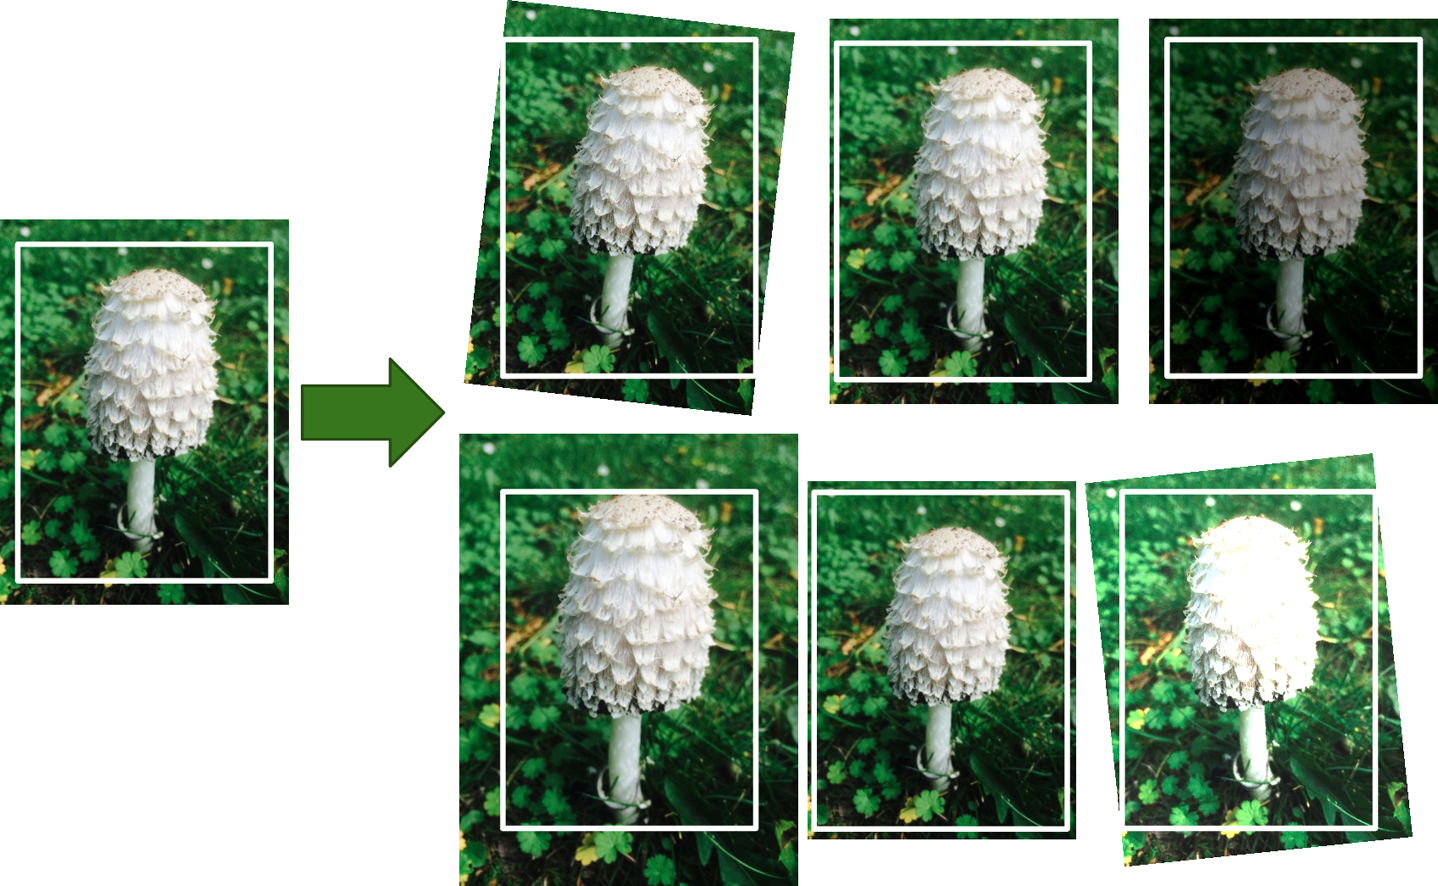
\includegraphics[width=0.6\textwidth]{images/dataAug}
  \caption{Aplicación de la técnica de Data Augmentation a una imagen de ejemplo \cite{book:homl}.}
  \label{fig:dataAug}
\end{figure}


Para aplicar esta técnica en nuestro caso, se puede aprovechar la API que proporciona Keras a tal efecto, por lo que no es necesario llevar a cabo la implementación. Es importante remarcar que el enfoque de Keras, en lugar de crear ejemplos mediante las transformaciones descritas, aplica solamente una transformación por imagen, lo que significa que no obtendremos una mayor cantidad de datos, pero sí que aumentará la variabilidad respecto a utilizar los datos en crudo.

\subsection{Selección de un modelo}

Este es visión mediante deep learning, por lo que lo lógico es que requiera de la potencia de una red neuronal convolucional. Sin embargo, algunos problemas pueden ser solucionados por un método más sencillo, por lo que podríamos probar con una red neuronal densa y constatar que no es suficiente para el problema en cuestión.

Utilizando una arquitectura de red mediante la que puede resolverse un dataset simple como es Fashion MNIST \cite{art:xiao2017fashionmnist}, se entrena un clasificador que nos da los resultados en la figura \ref{fig:dense}. Claramente, el modelo no es lo suficientemente potente como para aprender y tanto la precisión como la función de loss no varían con las épocas de entrenamiento (en la gráfica sólo se aprecian 10 debido a que se utilizó early stopping).

\renewcommand{\lstlistingname}{Código}
\begin{lstlisting}[caption={Arquitectura de la red densa.},captionpos=b]
_________________________________________________________________
Layer (type)                 Output Shape              Param #   
=================================================================
flatten_1 (Flatten)          (None, 9408)              0         
_________________________________________________________________
dense (Dense)                (None, 350)               3293150   
_________________________________________________________________
dense_1 (Dense)              (None, 350)               122850    
_________________________________________________________________
dense_2 (Dense)              (None, 350)               122850    
_________________________________________________________________
dropout (Dropout)            (None, 350)               0         
_________________________________________________________________
dense_3 (Dense)              (None, 2)                 702       
=================================================================
Total params: 3,539,552
Trainable params: 3,539,552
Non-trainable params: 0
_________________________________________________________________
\end{lstlisting}

\begin{figure}[h]
  \centering
  \begin{subfigure}[t]{0.4\linewidth}
    \centering
    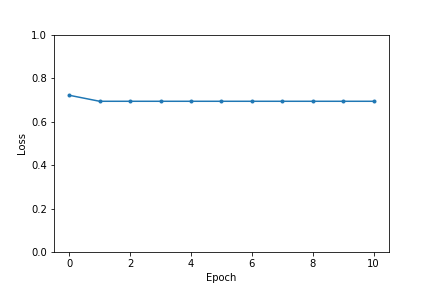
\includegraphics[height=4cm]{images/dense_loss.png}
  \end{subfigure}
  \begin{subfigure}[t]{0.4\linewidth}
    \centering
    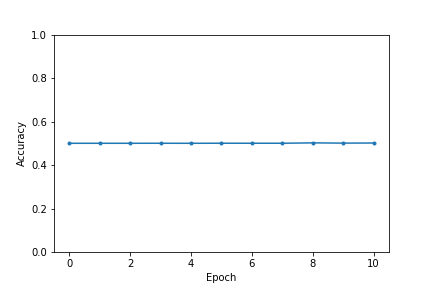
\includegraphics[height=4cm]{images/dense_acc.png}
  \end{subfigure}
  \caption{Resultados del entrenamiento de una red neuronal densamente conectada.}
  \label{fig:dense}
\end{figure}

En vista de los resultados, descartaremos este modelo y emplearemos un modelo convolucional. Lo mejor en este caso es utilizar un modelo de \textit{Fully Convolutional Network}, o FCN, dado que este tipo de modelos funcionan ante cualquier tamaño de entrada, con lo que no necesitamos aplicar ningún procesamiento especial cuando pasemos de predecir imágenes de 56x56 a predecir sobre cada uno de los frames del vídeo.

La estructura utilizada será la que puede verse en la tabla \ref{tabla:fcn}. Los tamaños utilizados en la tabla son los de una imagen de entrenamiento, aunque como hemos dicho, este modelo es capaz de procesar cualquier tamaño superior a 56x56. Cualquier imagen se vería reducida a razón de $\lfloor\frac{tam\_anterior - tam\_kernel}{strides}\rfloor+1$ en las capas P1, P2 y C4. Como podemos ver en la tabla, la capa C4 se comporta de la misma forma que lo haría una capa de aplanamiento, y es la que hace que no necesitemos añadir capas densas a esta arquitectura.

\begin{table}[h]
  \centering
  \begin{tabular}{|l|l|p{1.4cm}|p{1.4cm}|p{1.5cm}|l|l|p{1.4cm}|}
    \hline
    Capa    & Tipo      & Número de mapas & Tamaño de imagen & Tamaño del kernel & Stride & Padding & Función de activación \\ \hline
    Entrada & Input     & 3(RGB)          & 56x56            & -                 & -      & -       & -                     \\ \hline
    C1      & Conv2D    & 64              & 56x56            & 5x5               & 1      & same    & relu                  \\ \hline
    P1      & MaxPool2D & 64              & 27x27            & 3x3               & 2      & valid   & -                     \\ \hline
    C2      & Conv2D    & 256             & 27x27            & 3x3               & 1      & same    & relu                  \\ \hline
    C3      & Conv2D    & 256             & 27x27            & 3x3               & 1      & same    & relu                  \\ \hline
    P2      & MaxPool2D & 256             & 13x13            & 2x2               & 2      & valid   & -                     \\ \hline
    C4      & Conv2D    & 32              & 1x1              & 13x13             & 1      & valid   & relu                  \\ \hline
    Out     & Conv2D    & 1               & 1x1              & 1x1               & 1      & valid   & sigmoid               \\ \hline
  \end{tabular}
  \caption{Estructura de la red neuronal completamente convolucional}
  \label{tabla:fcn}
\end{table}

Tras entrenarla con los parámetros por defecto utilizando el optimizador Adam, obtenemos el resultado que puede verse en la figura \ref{fig:fcn}. Como puede verse, el modelo mejora al anterior aunque se puede apreciar una clara fluctuación en la función de loss y en la precisión. Para paliar este problema habrá que ajustar los hiperparámetros y aplicar técnicas de regularización.

Aún con la fluctuación, los resultados son claramente prometedores, con más de un 97\% de precisión, que podría mejorarse una vez ajustados los hiperparámetros

\begin{figure}[H]
  \centering
  \begin{subfigure}[t]{0.4\linewidth}
    \centering
    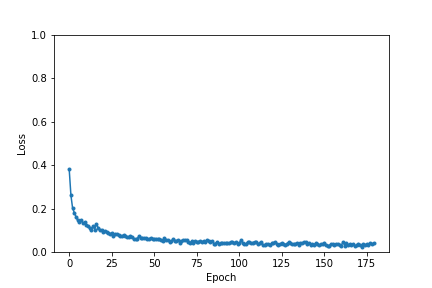
\includegraphics[height=4cm]{images/fcn_nohparam_loss.png}
  \end{subfigure}
  \begin{subfigure}[t]{0.4\linewidth}
    \centering
    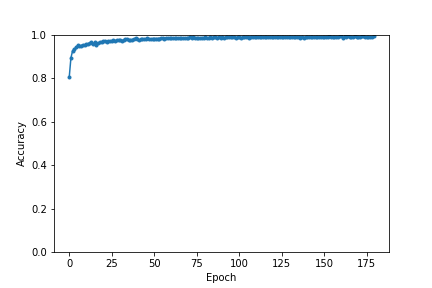
\includegraphics[height=4cm]{images/fcn_nohparam_acc.png}
  \end{subfigure}
  \caption{Resultados del entrenamiento del modelo FCN.}
  \label{fig:fcn}
\end{figure}


\subsection{Entrenamiento del modelo seleccionado}

Como hemos visto, los parámetros por defecto nos dan un buen modelo, pero aún podría mejorarse mediante técnicas de regularización y el ajuste de hiperparámetros. Los parámetros a retocar en el actual estado son el \textit{learning rate} del optimizador, e incluso los pesos de cada clase, dado que hay una cierta sobrerrepresentación en la clase negativa sobre la positiva.

Otro aspecto importante en el entrenamiento del modelo es el uso de la técnica de Early Stopping. Esta técnica consiste en detener el entrenamiento basándose en una serie de criterios sobre alguna de las métricas del entrenamiento. En este caso, se utiliza el valor de la función loss sobre el conjunto de validación. Si durante 50 épocas de entrenamiento no mejora dicha métrica en, al menos, $0.001$, se abandona el entrenamiento y se restauran los pesos de la iteración que mejor valor obtuviera.

Las ventajas de esta técnica son principalmente 2, primero acorta el tiempo de entrenamiento deteniéndolo en caso de no obtener mejoras durante un largo espacio de tiempo, lo cual es importante en el entrenamiento de redes neuronales convolucionales, que suelen tomar un tiempo considerable. Además, previene el sobreaprendizaje sobre el conjunto de entrenamiento, lo cual conduce a un peor resultado en los conjuntos de validación y test.

\subsubsection*{Ajuste de hiperparámetros}

El primer parámetro que ajustaremos es el \textit{learning rate} del optimizador puesto que podemos beneficiarnos de la estabilidad que proporcionaría este parámetro bien ajustado de cara a ajustar el resto de parámetros.

Dado que el valor por defecto ($10^{-3}$) estaba causando fluctuación en las métricas del entrenamiento, podemos utilizar valores más pequeños (en este caso, $10^{-4}$ y $10^{-5}$) que haga al modelo aprender más lentamente e intentar mantener la mejora de las métricas más estable. El resultado de este ajuste puede verse en los gráficos \ref{fig:lr_acc} y \ref{fig:lr_loss}. Como puede verse, los valores de $10^{-4}$ y $10^{-5}$ son más estables que el valor por defecto, pero siguen siendo parecidos entre sí. Dado que un valor más pequeño del parámetro suele hacer más lento el aprendizaje, lo mejor será utilizar $10^{-4}$ como valor para los siguientes procedimientos.

\begin{figure}[H]
  \centering
  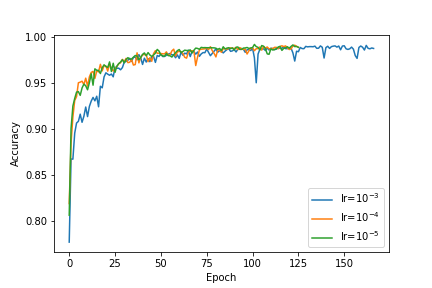
\includegraphics[width=0.7\textwidth]{images/lr_acc.png}
  \caption{Resultados del ajuste del parámetro \textit{learning rate} en la precisión del modelo.}
  \label{fig:lr_acc}
\end{figure}

\begin{figure}[H]
  \centering
  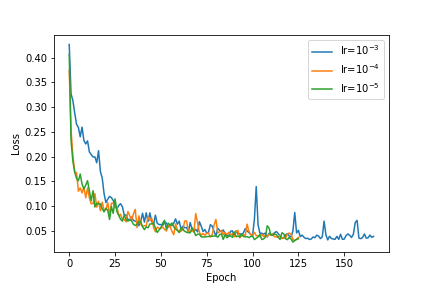
\includegraphics[width=0.7\textwidth]{images/lr_loss}
  \caption{Resultados del ajuste del parámetro \textit{learning rate} en la función de loss.}
  \label{fig:lr_loss}
\end{figure}

Con este nuevo valor en el parámetro del \textit{learning rate} nos queda ajustar los pesos de las clases, con el objetivo de lograr un aprendizaje mayor en la clase positiva, que se encuentra subrepresentada respecto a la negativa. Es razonable que exista esta desproporción, ya que en todos los frames es de esperar que solamente haya un positivo y el resto de la imagen sean negativos puesto que solo hay un balón. Sin embargo, si el objetivo es un modelo capaz de hacer detección desde cero del balón, necesitaremos que dé la menor cantidad de falsos positivos posible.

A fin de equiparar a ojos del modelo las importancias de las clases tanto positiva como negativa, debería compensarse la desproporción en cantidad de cada clase con los pesos asignados a estas. Dado que los ejemplos en el dataset son 6961 negativos por 2565 positivos, deberíamos asignarle a la clase positiva un peso de aproximadamente $2.5$ que asegure que el modelo les dé la misma importancia a ambas. El modelo resultante consigue los resultados de las figuras con una precisión sobre el conjunto de test del 99.47\%.

\begin{figure}[H]
  \centering
  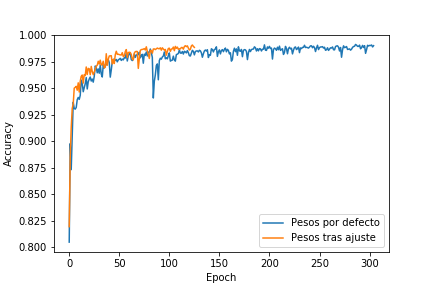
\includegraphics[width=0.7\textwidth]{images/cw_acc.png}
  \caption{Resultados del ajuste peso de las clases en la precisión del modelo.}
  \label{fig:cw_acc}
\end{figure}

\begin{figure}[H]
  \centering
  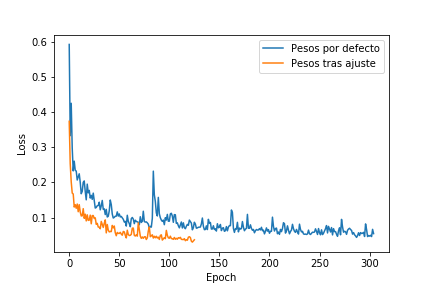
\includegraphics[width=0.7\textwidth]{images/cw_loss}
  \caption{Resultados del ajuste peso de las clases en la función de loss.}
  \label{fig:cw_loss}
\end{figure}

Como puede verse en las figuras \ref{fig:cw_acc} y \ref{fig:cw_loss}, el modelo da una métricas ligeramente peores en cuanto a loss y precisión. Sin embargo, este supuesto empeoramiento viene debido a una mejor generalización por parte del algoritmo de las clases negativa y positiva.

Esto se hace evidente al ver el desempeño sobre un vídeo real, mientras que el modelo previo a ajustar el peso de las clases tiende a fallar a la hora de identificar en balón en escena (falsos negativos), el modelo posterior al ajuste se mantiene consistente al identificar el balón, a costa de la aparición de algunos falsos negativos que tendremos que pulir.

Estos problemas pueden verse en la figura \ref{fig:vidcw}, en la que podemos ver la salida de ambos modelos en un vídeo real. Este es un caso típico donde el primer modelo falla mientras que el segundo es capaz de ubicar el balón. Por supuesto, no es ni mucho menos un modelo perfecto, pero aún podemos depurar estos falsos positivos como veremos en la siguiente sección.

\begin{figure}\centering
  \subfloat[Imagen original]{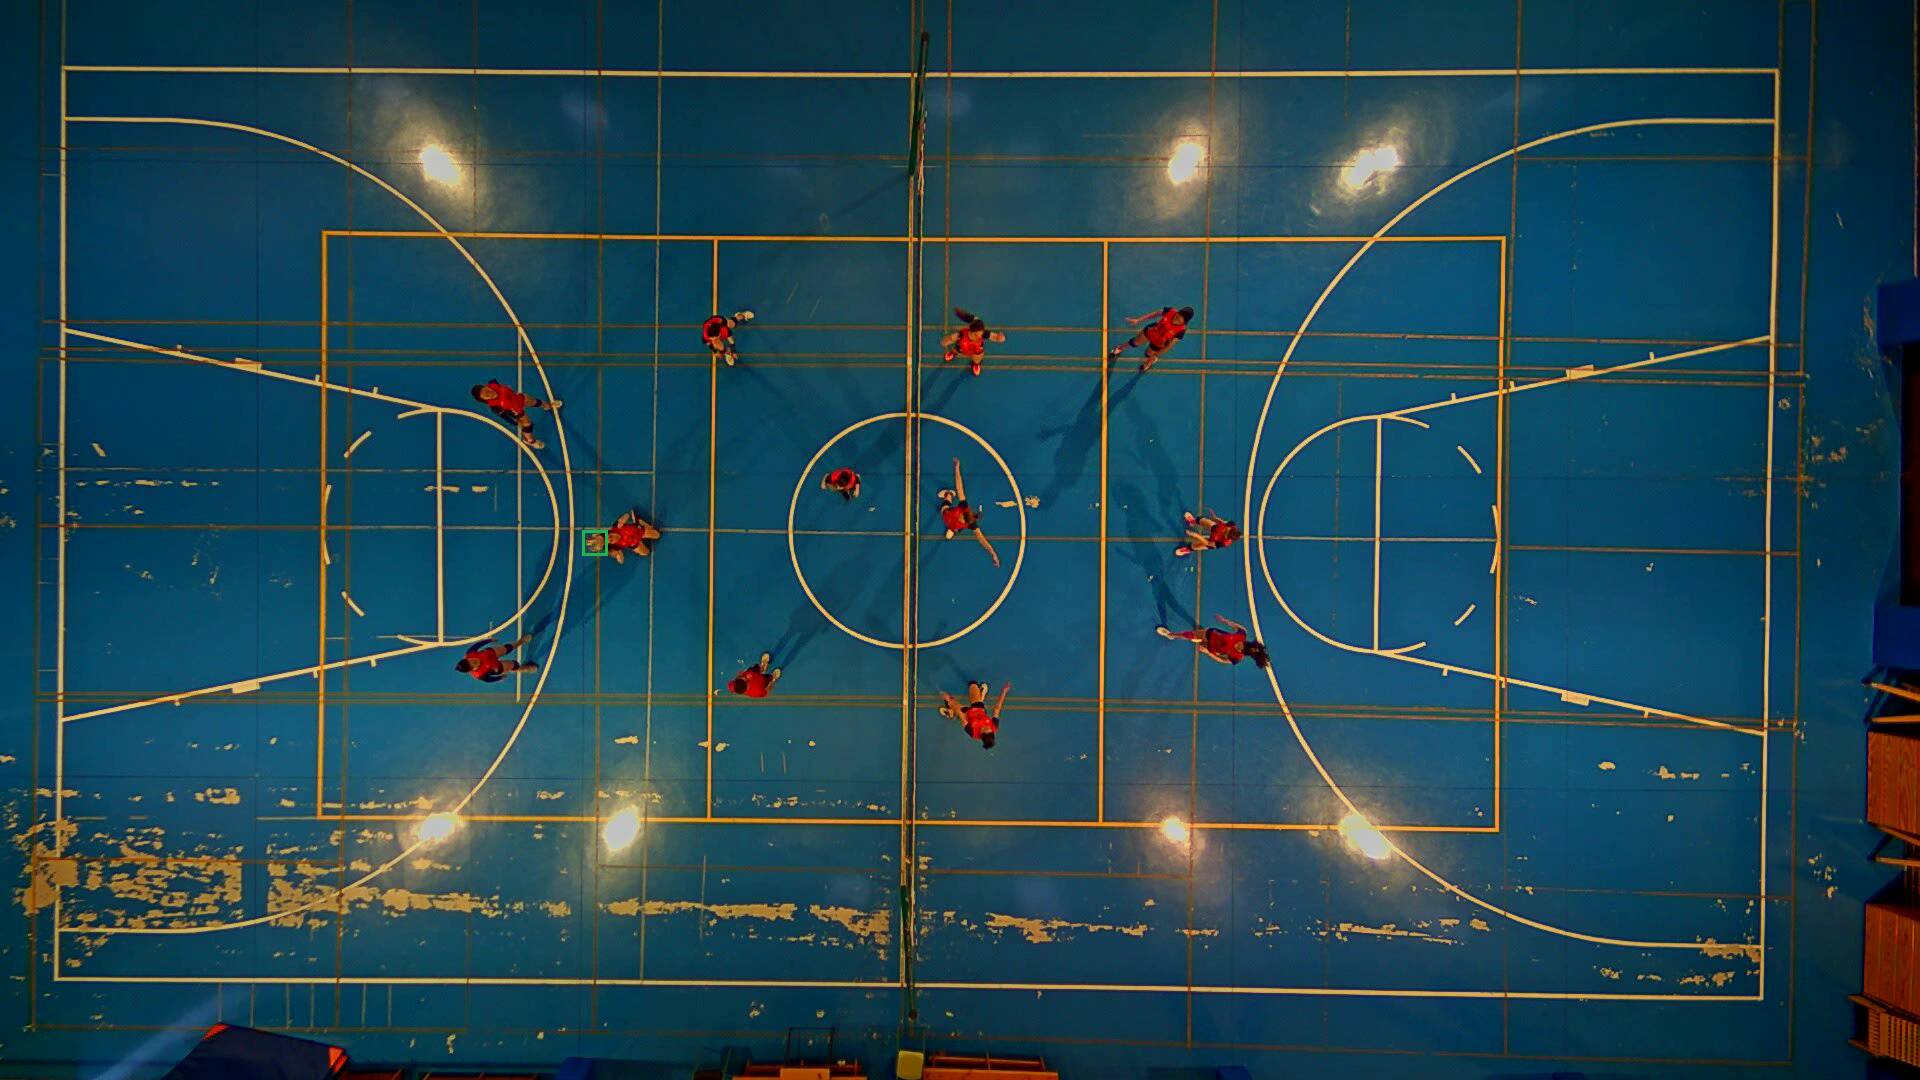
\includegraphics[width=.8\linewidth]{images/original.png}}\par
  \subfloat[Salida antes del ajuste de pesos]{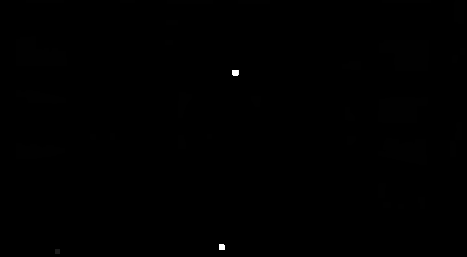
\includegraphics[width=.45\linewidth]{images/model1.png}}\hfill
  \subfloat[Salida después del ajuste de pesos]{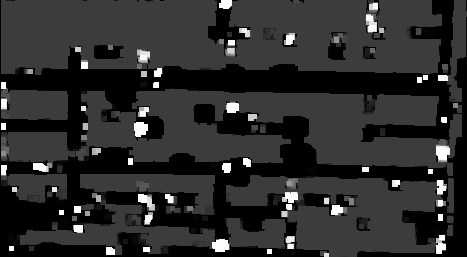
\includegraphics[width=.45\linewidth]{images/model2it0.png}}
  \caption{Comparativa entre los modelos resultantes antes y después de ajustar los pesos de las clases}
  \label{fig:vidcw}
\end{figure}

\subsubsection*{Hard negative mining}

El modelo que hemos obtenido tras este proceso adolece en cierta medida de un problema con los falsos positivos. Para reducir este problema, se puede aplicar una técnica llamada \textit{hard negative mining}. Esta técnica consiste en reutilizar los errores en vídeos reales (no en el dataset de entrenamiento) del algoritmo para realimentar el modelo, de forma que aprenda de sus errores a lo largo de una serie de iteraciones.

Nuevamente, este proceso no puede ser completamente automático, ya que necesita de un etiquetado con el \textit{ground truth} de dónde se encuentra el balón en cada frame del vídeo para saber qué positivos son errores y qué positivos son correctos. Una alternativa para esto sería utilizar un sistema de etiquetado frame a frame para cada vídeo, pero queda fuera del alcance del presente trabajo.

En su lugar, se tomará una serie de imágenes aleatoriamente de los vídeos y, tras etiquetar a mano las posiciones se usarán como fuentes para los falsos positivos (y falsos negativos). Una vez identificados los errores del modelo, se obtienen los parches de 56x56 y se reintroducen en el dataset, volviendo a dividirlos en subconjuntos de entrenamiento, validación y test.

Hay un par de aspectos importantes a considerar en esta tarea, el primero de los cuales es que los parches que recojamos no pueden estar localizados en el mismo lugar en la imagen original, puesto que esto los haría ser idénticos y, al hacer la división en los subconjuntos, hay una posibilidad de que imágenes idénticas acaben en subconjuntos distintos, contaminando el dataset. Para evitar este problema, se comprueba que cada parche está a más de 20 píxels de todos los existentes, no solo de esa imagen, sino de todas las que utilicemos.

Hay que tener en cuenta que la salida del modelo no es una imagen del mismo tamaño que la imagen de entrada, sino que se ve reducida, como decíamos anteriormente, a razón de $\lfloor\frac{tam\_anterior - tam\_kernel}{strides}\rfloor+1$ en 3 capas del modelo. Esto significa que la imagen se transforma en tamaño a razón de $\lfloor\frac{(\lfloor\frac{x-3}{2}\rfloor + 1)}{2}\rfloor-12$, lo cual quiere decir que una imagen de 1920x1080 como las de los vídeos originales se convierte en una imagen de 467x257. Debido a esto, necesitamos calcular la posición en las imágenes originales de los positivos del modelo (entendiendo cada \textit{cluster} de positivos como un contorno).

En los problemas de segmentación semántica se acostumbra a utilizar capas de reconstrucción al final de la arquitectura de la red, pero en nuestro caso no es necesario complicar el modelo ya que solo necesitamos calcular la posición exacta. Esto se puede hacer mediante la siguiente fórmula $x_{in},y_{in} = x_{out} * 4, y_{out} * 4$, lo cual nos daría la esquina superior izquierda del rectángulo que ha producido esa salida. Para obtener la esquina inferior derecha, solamente hay que sumar 55 en ambas coordenadas.

Una vez se obtienen todos los errores candidatos a reintroducir al dataset, los dividimos en la misma proporción que este ($0.80$ entrenamiento, $0.1$ test y $0.1$ validación). Dado que este es un proceso iterativo, cada modelo tendrá una carpeta por iteración en el sistema de ficheros, y para evitar que con el curso de muchas iteraciones se acabe utilizando demasiado espacio en disco, los ejemplos de iteraciones anteriores se añaden como enlaces simbólicos.

Además, con solamente añadir los falsos positivos o negativos al dataset no es suficiente, puesto que con el paso de unas cuantas iteraciones, eso llevará a un desbalanceo de clases porque los falsos positivos son siempre más comunes que los falsos negativos (dado que solo hay un balón en la escena, por tanto solo puede haber un falso negativo o ninguno). Para evitar este problema se eliminan tantas imágenes del dataset como se vayan a introducir. Es decir, si vamos a introducir 60 negativos al conjunto de entrenamiento se eliminan otros 60 negativos que existieran previamente.

Cuando tenemos la nueva carpeta con los errores del modelo, se carga y se reentrena con los mismos parámetros de entrenamiento que se han usado previamente hasta lograr un mejor modelo que en la iteración anterior. Aunque no hay limitación de cuántas iteraciones pueden hacerse, normalmente es suficiente con no más de 2 o 3 para depurar el modelo hasta cierto punto.

\begin{figure}\centering
  \subfloat[Imagen original]{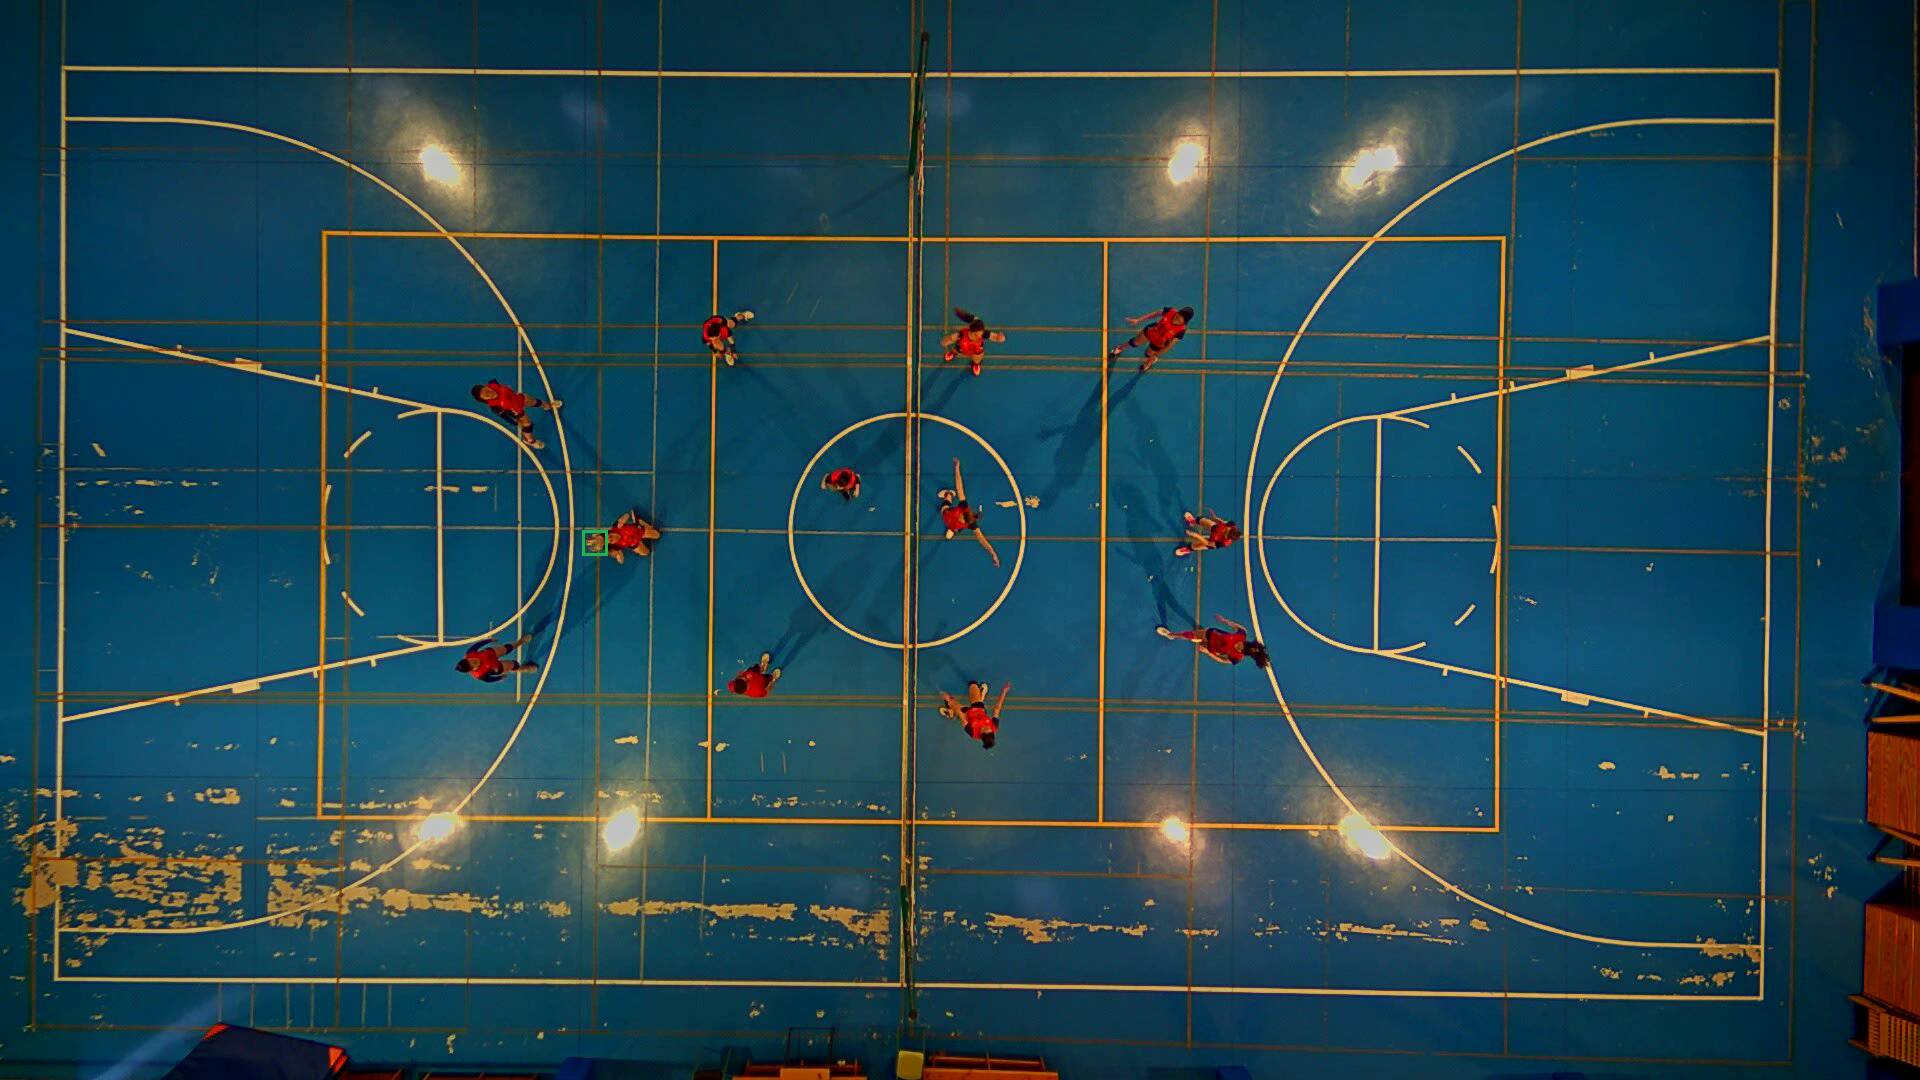
\includegraphics[width=.8\linewidth]{images/original.png}}\par
  \subfloat[Salida antes de aplicar Hard Negative Mining]{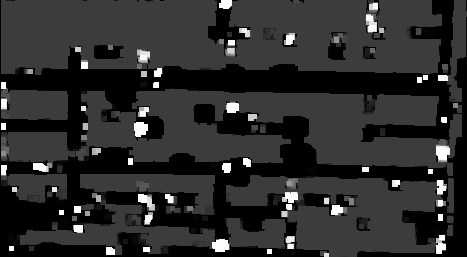
\includegraphics[width=.45\linewidth]{images/model2it0.png}}\hfill
  \subfloat[Salida después de aplicar Hard Negative Mining]{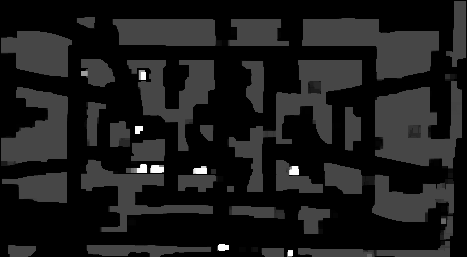
\includegraphics[width=.45\linewidth]{images/model2it2.png}}
  \caption{Salida del modelo antes y después de una iteración de Hard Negative Mining.}
  \label{fig:hnmining}
\end{figure}

En la figura \ref{fig:hnmining} vemos la salida tras la primera iteración de Hard Negative Mining, donde se ve que los falsos positivos están mucho mejor controlados. Aún se aprecian algunos falsos positivos que tendremos que manejar utilizando heurísticas.

\subsubsection*{Evaluación del modelo en un entorno real}

La evaluación del modelo en un entorno real, es decir, sobre un vídeo, es una tarea que de forma óptima se haría etiquetando a mano cada uno de los frames del vídeo con la posición del balón, y entonces podríamos utilizar la métrica Intersection over Union (IoU), la cual indica el grado de acierto del modelo a la hora de posicionar en este caso la pelota en la escena.

\begin{figure}[H]
  \centering
  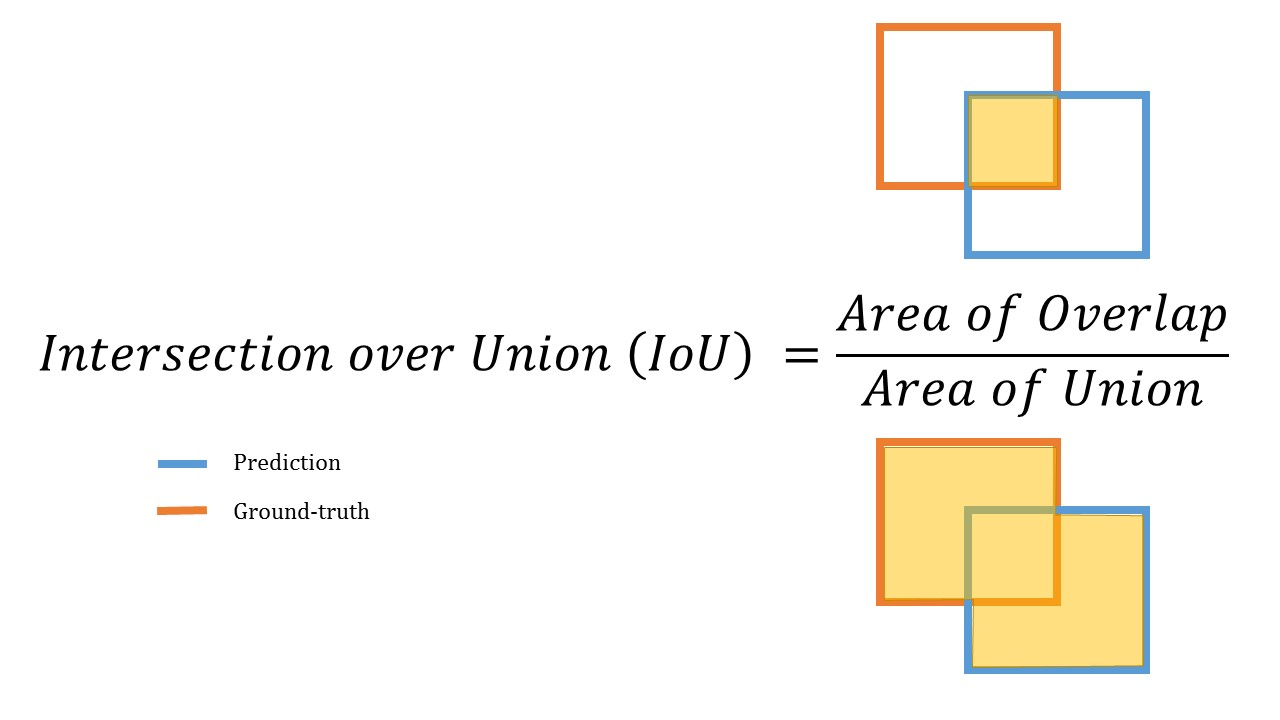
\includegraphics[width=0.7\textwidth]{images/IoU.jpg}
  \caption{Visualización de la métrica IoU \cite{kaggleIoU}.}
  \label{fig:IoU}
\end{figure}

Por la envergadura de esta tarea, queda fuera del alcance de este trabajo. En su lugar se ha optado por una forma de medir mas ``a ojo'', donde nos fijaremos en cuántos frames de una jugada es capaz el modelo de detectar el balón desde cero. Es importante remarcar que, dado que hay una cierta cantidad de falsos positivos, le introduciremos al modelo una región de interés (ROI) que servirá como punto de partida para la detección, con esto evitando otros positivos que pueda haber en la escena. Además, el seguimiento del balón se hará moviendo una ventana en la dirección de su movimiento una vez detectado, en lugar de procesar todo el frame cada vez.

Utilizaremos para la comparativa los modelos final tras ajustar los parámetros y el obtenido después de pasar el primero por unas pocas iteraciones de Hard Negative Mining.

\subsection{Descripción del software final}

En esta sección se explicarán todos los scripts importantes de cara al proceso de entrenar el modelo y evaluarlo. Todos estos scripts se ejecutan utilizando la línea de comandos.

\subsubsection*{Entrenar el modelo}

El script \textbf{classifier.py} controla el entrenamiento del modelo. Este script tiene como parámetro la ubicación del dataset. Al ejecutarlo, lee los subdirectorios que cuelgan de dicha ruta, que deben ser 3: train, test y val, es decir, los directorios de entrenamiento, test y validación. Utilizando dichos datos, se entrena el modelo hasta que el entrenamiento se detenga por el \textit{early stopping}, dándonos la metrica de precisión en el conjunto de test y preguntando si queremos guardar el modelo entrenado. Si seleccionamos ``Sí'', se guarda el modelo en el directorio \textit{models}.

\subsubsection*{Hard Negative Mining}

Para aplicar esta técnica se utiliza el script \textbf{retrain.py}, que a su vez ejecuta otros dos scripts \textbf{hnExtraction.py} y \textbf{hnMining.py}. De ellos, el primero obtiene los parches de entrenamiento a partir de los falsos positivos y el segundo utiliza el dataset resultante para volver a entrenar el modelo. El modelo resultante del script se guarda en el fichero models con el nombre itxnombre.h5 donde x es el número de iteración de la técnica y nombre es el nombre original del modelo.

Este script recibe los siguientes parámetros:

\begin{itemize}
  \item \textbf{Modelo.} Argumento posicional que es la ruta del modelo al que queremos aplicar la técnica.
  \item\textbf{-r o --refs.} Argumento opcional donde se le indica al script la localización de las imágenes de donde obtendremos los falsos positivos y negativos.
  \item \textbf{-i o --iterations.} Argumento opcional con el número de iteraciones que queremos aplicar. El valor por defecto es 5.
  \item \textbf{-d o --data.} Argumento opcional donde indicamos la localización del dataset. Este argumento solamente es necesario en la primera iteración dado que en las demás se obtiene a partir del nombre del modelo y su número de iteración. En la segunda y sucesiva iteraciones es ignorado.
\end{itemize}

\subsubsection*{Probar el modelo final en un vídeo real}

Para ver la salida del modelo en un vídeo real, se utiliza el script \textbf{tracker.py}, al cual se le pasa un modelo y un vídeo, y muestra este último junto a la salida del modelo. Además, se dibuja un rectángulo sobre el balón en la imagen del vídeo original, en concordancia con la posición predicha por el modelo.

Para iniciar el seguimiento, se debe pulsar la tecla ``t'', ante lo cual se abrirá una ventana para seleccionar una ROI que servirá como punto de partida para la detección.

\newpage